\section{Evaluation}
\label{sect:evaluation}
We have implemented and evaluated a prototype of our VC scheme on a Linux cluster of machines with
8-core 3.1Ghz AMD FX-8120 and 16 GB RAM. 
Our implementation is based on the Alibaba cloud platform~\cite{Aliyun,WeiZhangIEEE}
and the underlying DFS uses  QFS with default replication degree 3 while the PDS replication degree is 6.
Our evaluation objective is to
study deduplication efficiency and resource usage of VC,  
and assess its processing time and backup throughput, and  
the benefit in fault tolerance. 
We will compare VC with a VO approach  using stateless routing with binning (SRB) 
based on~\cite{Dong2011,extreme_binning09}.
SRB executes distributed deduplication by routing data chunks to cluster machines~\cite{Dong2011}
using  a min-hash function discussed in \cite{extreme_binning09}. Once a data chunk is routed to
a machine, the chunk is compared with the fingerprint index within this machine locally based 
on~\cite{extreme_binning09}.

%{\bf Settings}.
We have performed a trace-driven study based on a production dataset
from Alibaba Aliyun's cloud platform~\cite{Aliyun} 
with about 2500 VMs, running on 100 physical machines. 
Each machine in the production environment is more powerful than our evaluation cluster
and has 16 cores with 48GB memory.
Each machine hosts up to 25 VMs and each VM keeps 10 automatically-generated snapshots in the storage 
system while a user may instruct extra snapshots to be saved.
Each VM has about 40GB of storage  data  on average
including OS and user data disk while the size distribution is highly skewed and the maximum to
the average ratio is close to 40.
Each physical machine deals with about 10TB of snapshot data and each 1TB data represents one snapshot version
of 25 VMs.  Thus the total amount of raw snapshot shot in 100 physical machines
is about 1,000TB.
The VMs of the sampled data set use popular operating systems such as 
Debian, Ubuntu, Redhat, CentOS, win2008 and win2003. 
%The backup of VM snapshots is required to complete within few  hours every night.
The daily snapshot change rate is about 2-3\% on average.
%All data are divided into 2 MB fix-sized segments and 
The fingerprint for variable-sized chunks is computed using their SHA-1 hash~\cite{similar94,rabin81}. 
%Each segment is divided into 
%variable-sized content chunks with an average size of 4KB.
%Popularity of data blocks are collected through global counting and 
%and top popular ones ($\delta=2\%$)  are  kept in the PDS, as discussed in Section~\ref{sect:store}.

\subsection{Deduplication Efficiency and Memory Usage}
\label{sect:evaldedup}


\comments{
\begin{figure}[htb]
    \centering
    \begin{tikzpicture}
        \begin{axis}[
                width=\linewidth,
                height=0.6\linewidth,
                ybar,
                bar width=0.5cm,
                ymax=98.7,
                enlarge x limits=0.15,
                style=thin,
                ylabel={Dedup. Efficiency (\%)},
                ytick={93,94,95,96,97,98},
                xtick=\empty,
                ymajorgrids,
                grid style=densely dotted,
                %symbolic x coords={VC-No PDS, VC-2\%PDS w/o similarity, VC-2\%PDS, VC-4\%PDS, SRB},
                %symbolic x coords={VC0, VC2N, VC2, VC4, SRB},
                %xticklabels from table={figures/efficiency_comparison_bars.txt}{alg}
                nodes near coords,
                every node near coord/.append style={
                    anchor=-145+\coordindex*10
                }
            ]
            %\addplot[fill=blue] coordinates {(VC0,93.02) (VC2N,94.31) (VC2,96.01) (VC4,96.58) (SRB,97.86)};
            %\addplot[fill=blue] coordinates { (VC-No PDS,93.02) (VC-2\%PDS w/o similarity,94.31) (VC-2\%PDS,96.01) (VC-4\%PDS,96.58) (SRB,97.86) };
            \addplot [%
                point meta=explicit symbolic,
                fill=blue
            ] table [x expr=\coordindex, y=efficiency,meta=alg] {figures/efficiency_comparison_bars.txt};
        \end{axis}
    \end{tikzpicture}
    \caption{Efficiency comparison between different VC settings and
        Stateless Routing with Binning}
    \label{fig:efficiency-comparison}
\end{figure}
}

\comments{
alg     efficiency
\scriptsize{}VC-2\%\tiny{}No\ Similarity        94.3132243792193
\scriptsize{}VC-NoPDS   93.0202119345744
\scriptsize{}VC-2\%PDS  96.0127647380588
\scriptsize{}VC-4\%PDS  96.5784837160482
\scriptsize{}SRB        97.8625610883421
}


\comments{
old table, delete 4%
    \begin{tabular}{|c|c|c|c|c|c|}
    \hline 
&
     \multicolumn{4}{|c|}{VC}  & VO \\ \hline
&
     2\%PDS  &  No PDS &2\%PDS     & 4\%PDS & SRB  \\ 
&     no-simi&   &&  &    \\ \hline
Dedup &     94.31\%& 93.02\%  & 96.01\% & 96.58\% & 97.86\% \\ \hline
Mem(MB) &     108&  46 & 118  & 190 & 2400 \\ \hline
    \end{tabular}

}
\begin{table}[htb]
\centering
    \begin{tabular}{|c|c|c|c|c|}
    \hline 
&
     \multicolumn{3}{|c|}{VC}  & VO \\ \hline
&
     2\%No PDS &2\%PDS     & 2\%PDS & SRB  \\ 
&        &&     no-simi & \\ \hline
Dedup &      93.02\%  & 96.01\% & 94.31\% & 97.86\% \\ 
Efficiency &          &       &           &      \\    \hline 
Memory &      10MB & 118MB  & 108MB & 2.4GB \\ 
per-machine &      &   &  &  \\ \hline
    \end{tabular}
    \caption{Deduplication efficiency and per-machine memory usage for different VC settings and
        Stateless Routing with Binning (SRB).}
    \label{tab:efficiency-comparison}
\end{table}


Table~\ref{tab:efficiency-comparison} shows the deduplication efficiency and per-machine memory usage for SRB and VC with different 
settings.
% <<<<<<< HEAD
% Our deduplication efficiency is defined as the percent of duplicate chunks
% which are detected and deduplicated, so only global perfect deduplication can have 100\% efficiency.
% The figure also compares several PDS sizes chosen for VC. ``$\sigma=2\%$'' 
% is defined in Table~\ref{tab:symbol}. 
% =======
Deduplication efficiency is defined as the percent of duplicate chunks which are removed
compared to a perfect scheme which detects and removes  all duplicates. 
% so only global perfect deduplication can have 100\% efficiency.
% We also compare several PDS sizes chosen for VC.
%(see Table~\ref{tab:symbol} for definition of ``$\sigma=2\%$'')
%we allocate the space of distributed shared memory  to accommodate 2\%
%of data chunks shared among VMs, as defined in 
Notice $\sigma$ is the percentage of unique chunks selected in PDS.
With $\sigma =2\%$, Column 3 shows its 
%memory usage for PDS index lookup per machine is about 100MB per machine and  the 
deduplication efficiency can 
reach over 96\%. 
%When $\sigma=4\%$, Column 4 shows that the deduplication efficiency can reach 96.6\% while 
%more index space is allocated  per machine for  PDS fingerprint lookup.
The loss of efficiency in VC is caused by the restriction of the physical memory available
in the cluster for fast in-memory PDS index lookup. 
Memory usage per machine is low because each machine only hosts $1/p$  of  index for PDS 
plus some buffer space where $p$ is the number of physical machines. 
%In the extreme case if we put all the fingerprint into PDS 
%index ($\sigma=100\%$) then VC will have 100\% efficiency.
SRB in Column 5 can deliver up to 97.86\% deduplication efficiency, which is slightly better than VC.
Thus this represents a tradeoff as VC uses much less resource  and faster deletion.
%with a slight reduction in deduplication efficiency.
Memory usage per machine in SRB includes the Bloom filter space to access the on-disk index
and  cache for frequently or recently accessed chunk index.  
% SRB can deliver up to 97.935\% deduplication efficiency which is slightly better than VC.
% Thus this represents a tradeoff: VC provides better fault tolerance and fast
% approximate deletion with competitive (but slightly lower) deduplication
% efficiency.
% >>>>>>> 4dcd68612b052c0f890ed30361a9ed03771b5df1
%its loss of efficiency is caused by the routing of data chunks which restricts the search scope
%of duplicate detection.
%SRB provides slightly better deduplication efficiency than our VC approach, which we accept
%because we are rewarded by architecture-wise benefits such as fault-tolerance and fast 
%Though not our primary goal, this result does show that VC can remove competitive amount of duplicates.

Column 2 of Table~\ref{tab:efficiency-comparison} shows deduplication efficiency of VC without 
using PDS and it achieves 93.02\% and  missed duplicates take  up-to  3.56\% of the original space, which
is about 356GB per physical machine. 
Column 4 of Table~\ref{tab:efficiency-comparison} shows deduplication efficiency of VC which only uses
the same offset in the parent segment to look for duplicates  but does not look for other potentially
similar segments. 
%There is a big efficiency drop in this curve when the number of VMs is about 30.
We explain why similarity-guided local search provides such an improvement as follows.
%Without this (i.e. when we only 
There are VMs in which data  segments are moved to another location on disk, for example 
when a file is rewritten
rather than modified in place,  
and a dirty-bit or offset-only based detection would not be able to detect such a movement.
We have found that in
approximately 1/3 of the VMs in our dataset this movement happens frequently.
In general, adding local similarity-guided search increases deduplication efficiency from 94\% to over 96\%.
That is one significant improvement compared to the work in ~\cite{WeiZhangIEEE}
which uses the parent segment at the same offset to detect duplicates instead of similarity-guided search.
% In general, our experiments show that
% dirty-bit detection at the segment level can reduce the data size to about 24.14\% of original data, 
% which leads about a 75.86\% reduction.
% Similarity-guided local search can further reduce the data size
% to about 12.05\% of original size, namely it delivers an additional 12.09\% reduction.
% The PDS-based global duplicate detection with $\sigma=2\% $
% can reduce the size further to 8.6\% of original size, namely it 
% delivers an additional 3.45\% reduction.

In summary, our experiments show that
version detection at the segment level can reduce the data size to about 24.14\% of original data, 
which leads to about a 75.86\% reduction. Namely 10TB snapshot data per machine is reduced to 2.414TB.
Similarity-guided local search can further reduce the data size
to about 1.205T, which is  12.05\% of original. Thus it delivers a 50.08\% reduction after the version-based
 deduplication.
The popularity-guided global deduplication with $\sigma=2\% $
reduces the data further to 860GB, namely 8.6\% of the original size. 
So it provides additional 28.63\% reduction. 
The overall memory usage of VC for each physical machine is very small, which is insignificant to other 
hosted cloud services.  In comparison, the 2.4GB per-machine memory usage of SRB is very visible 
to other services.
% even each physical machine in the production environment has 48GB memory.

%Figure~\ref{fig:exbin-efficiency-graph2} also shows the benefits of our minhash
%similar segment search in the parent snapshot. 

Comparing the experiment results of the sampled index method reported in~\cite{Guo2011}, 
our scheme achieves a 85K:1 ratio between raw snapshot data and memory usage 
with 96\% deduplication efficiency
while the sampled index method achieves 20K:1 (10GB memory per 500TB raw data)
with 97\% deduplication efficiency.
Thus our scheme is more memory efficient with a good tradeoff for deduplication efficiency.
If we change $\sigma=4\%$, the deduplication efficiency of VC increases to 96.58\% while
memory usage per machine increases to about 220MB. 
Notice that the sampled index method is designed for single-machine deduplication.
%and it is not easy to extend to a distributed cluster architecture.


\subsection{More on Resource Usage and Processing Speed}

We show  additional experimental results on resource usage, processing time and throughput of VC.
\comments{
\begin{table}
    \begin{tabular}{|c|c|}
    \hline
    PDS replication degree & Disk usage per machine  \\ \hline
    3                      & 3065GB             \\ \hline
    4                      & 3072GB             \\ \hline
    5                      & 3079GB             \\ \hline
    6                      & 3086GB             \\ \hline
    7                      & 3093GB             \\ \hline
    \end{tabular}
\caption{Storage space cost per machine for DFS under different PDS replication degree}
\label{tab:replication_cost}
\end{table}
}

{\bf Storage cost of replication.} 
%Table ~\ref{tab:replication_cost} shows the total storage space required by 
%VC as the PDS replication degree changes while non-PDS replication degree is fixed as 3. 
When the replication degree of both PDS and non-PDS data is 3, 
the total storage  for all VM snapshots in each physical machine takes about 3.065TB on average before compression
and 0.75TB after compression.  Allocating  one extra  copy for PDS data only adds  7GB in total per machine.
Thus PDS replication degree 6 only increases the total space by 0.685\% while PDS replication degree 9 adds 1.37\% 
space overhead, which is still small.
%The increase in storage cost is minimal because the PDS makes up a 
%small percent of the total storage space, while increasing replication degree has a  more significant benefit for
%availability as shown in Figure~\ref{fig:pds-replication}.

\begin{table}
    \begin{tabular}{|c|c|c|c|c|c|}
    \hline
    Tasks & CPU & Mem &Read &  Write  & Backup Time  \\ 
    & & (MB)          &(MB/s) &  (MB/s) & (hrs) \\ \hline
%    1     & 19\% & 118.1 & 50MB/s 8.37 & 1.314\\ \hline
    1     & 19\% & 118 & 50 & 16.4 & 1.31\\ \hline
%    2     & 35\% & 131.8 & 9.0 & 1.226\\ \hline
    2     & 35\% & 132 &50  & 17.6 & 1.23\\ \hline
    %4     & 63\% & 154.1 & 9.3 & 1.179\\ \hline
    4     & 63\% & 154&50   & 18.3 & 1.18\\ \hline
    6     & 77\% & 171.9 & 50 &  18.8 & 1.162\\ \hline
%    8     & 82\% & 90.5 & 89.2 & \\ \hline
%    10                      & 85\% & 97.2   & 90.4 \\ \hline
%    12                      & 91\% & 95.6    & 91.5 \\ \hline
    \end{tabular}
\caption{Resource usage of concurrent backup tasks at each physical machine with $\sigma=2\%$ and I/O throttling.}
\label{tab:resource_usage}
\end{table}

{\bf Memory usage with multi-VM processing and disk bandwidth with  I/O throttling}. 
We have further studied the memory and disk bandwidth usage 
when running concurrent VM snapshot backup on each machine with $\sigma=2\%$. 
Table ~\ref{tab:resource_usage} gives the resource usage  when
running 1 or multiple  VM backup tasks at the same time on each physical machine. 
Each task handles the backup of one VM snapshot including deduplication.
``CPU'' column is the percentage of a single core used. 
``Mem'' column includes $\sim$100MB memory usage for PDS index and other space cost for executing deduplication tasks such as 
recipe metadata and cache. 
The ``Read'' column is controlled to 50MB/s local disk bandwidth usage with I/O throttling so that other 
cloud services are not significantly impacted.
The peak raw storage read performance is about 300MB/s and we only use 16.7\% with this collocation consideration.
``Write'' is the I/O write usage of QFS; note that each QFS write triggers disk writes in multiple machines due to
data replication.     50MB/s dirty segment read speed triggers about 16.4MB/s disk write for non duplicates with one backup task.
% [ NOT REASONABLE: Notice that memory and CPU used by PDS index and QFS are not included since they belong to 
% the cloud infrastructure services and are shared among many applications.]
%We see our hybrid deduplication scheme only occupies a small amount of system resources. 
%The  local deduplication only needs to keep the parent snapshot recipe and a few similar segment recipes in 
%memory during duplicate detection.

Table ~\ref{tab:resource_usage} shows that when  each machine conducts
backup one VM at a time, the backup of the entire
VM cluster completes in about 1.31 hours. Since there are about 25 VMs per machine, we could execute
more tasks in parallel at each machine. But adding more backup concurrency does 
not shorten the overall time
significantly in this case because of the controlled  disk read bandwidth usage.
When I/O throttling is not used, we will show below that processing multiple VMs concurrently 
does improve the throughput of backup.
%,  we can still process raw data at near 175 MB/s. If we consider the extreme case in which each machine has 25 VMs
%at 40GB size, our snapshot system can finish backing up all the VMs (1TB total) in 1.58 hours.


\comments{
It should be noted that global fingerprint  space requirement of VC is 2\% of all unique fingerprints 
with $\sigma$=2\%. SRB uses an approximated method to look for a match within a bin and
its memory space usage is about 190MB per machine. That is compared with 118MB used in VC with $\sigma=2\%$.
Using a bloom filter with an index cache would require more memory space~\cite{Dong2011}.
}
 
\comments{
The total memory space would cost over 6GB per machine.
We have implemented a bloom-filter for SRB which uses a comparable in-memory
index space size per machine compared VC, but SRB also needs extra space for caching hot index.
The total space used in SRB is about 1GB per machine. 
}

{\bf Processing time breakdown without I/O throttling}.
Table~\ref{tab:vc_srb_combined} shows
the  average  time breakdown for processing a dirty VM segment in milliseconds
under VC and Stateless Routing with Binning (SRB). 
%VC uses $\sigma=2\%$ and $4\%$.
VC uses $\sigma=2\%$. 
The overall processing latency of SRB is about 23.9\% slower than VC.
For VC, the change of $\sigma$ does not significantly affect the overall backup speed as
PDS lookup takes only a small amount of time. 
It has a breakdown of processing time.
``Read/Write'' includes snapshot reading and writing from disk, and 
updating of the metadata.
``Network'' includes the cost of transferring raw and meta data from one machine to another during 
snapshot read and write.
``Index Lookup'' is the disk, network and CPU time during fingerprint comparison.
This includes PDS data lookup for VC and index lookup from disk in SRB. 
The network transfer time for VC and SRB is about the same, because the 
amount of raw data they transfer is comparable.
SRB spends slightly more time for snapshot read/write because during each snapshot  backup, SRB involves many small bins,
 while VC only involves few containers with a bigger size. Thus, there are more opportunities for I/O aggregation in VC to reduce seek time.
SRB also has a higher cost for index access and fingerprint comparison because most chunk fingerprints are routed
to remote machines for comparison while   VC handles most chunk fingerprints locally. 

%on the index holding machine to access its index (often on the disk, supported by a Bloom filter) 
%and perform comparison.
%VC is faster in this regard because it conducts in-memory local search first and then
%accesses  the PDS on distributed shared memory, so most chunks can be dealt with locally.  
%SRB spends  slighter more time in  reading data and updates because it also updates the on-disk
%local meta data index in addition to partition indices.
%As a result Overall,  VC is faster than SRB, though data reading dominates the processing time for both algorithms.
%Figure~\ref{fig:vc_srb_combined} also reports the average backup time for a VM in VC when
%varying the PDS size.  It lists the time distribution for data reading,
%similarity-guided local search, global PDS lookup, and non-duplicate data writing. 
%While data reading dominates the backup process, PDS lookup spends about a similar amount
%of time as local search.

\begin{table}[t]
  \centering
    \footnotesize
    %\tabcolsep=0.11cm
    \pgfplotstabletypeset[
        comment chars=!,%use ! before a row in the data table to exclude it
        col sep=tab,
        %columns={Algorithm,Snapshot Read/Write,Network Transfer,Index access and comparison},
        columns={Algorithm,ReadWrite,Network,Index},
        columns/Algorithm/.style={
            string type,
            column name={\multirow{2}{*}{Algorithm}}
        },
        columns/ReadWrite/.style={
            column name={
                \multicolumn{3}{c|}{Time Spent in Task (ms)}\\&
                Read/Write
            },
            multiply by={1000},
            %preproc cell content/.code={1#1 1},
            fixed, precision=3
        },
        columns/Network/.style={
            column name={Network},
            multiply by={1000},
            fixed, precision=3
        },
        columns/Index/.style={
            column name={Index Lookup},
            multiply by={1000},
            fixed, precision=3
        },
        every head row/.style={
            before row={\hline},
            after row={\hline},
        },
        every last row/.style={after row=\hline},
        column type/.add={}{|},
        every first column/.style={column type/.add={|}{}},
    ]{figures/vc_srb_combined_pgfplots.txt}
    \caption{Average time in milliseconds  to backup a dirty 2MB VM segment under SRB and VC with I/O throttling.
%        \todo{Decide between this and bar plot with the same caption}
    }
    \label{tab:vc_srb_combined}
\end{table}

%\begin{figure}[htbp]
%  \centering
%  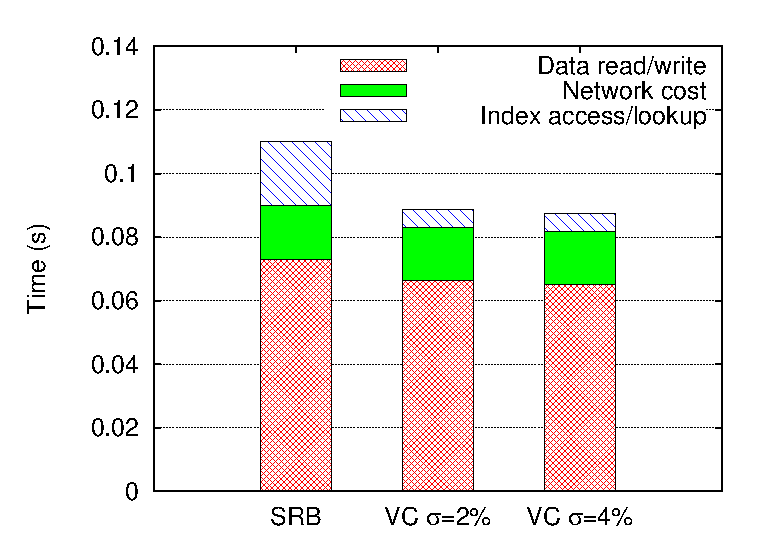
\epsfig{file=figures/vc_srb_combined, width=3in}
%  \caption{Average time to backup a dirty VM segment under SRB and VC}
%  \label{fig:vc_srb_combined}
%\end{figure}

% \begin{figure}[htbp]
%   \centering
%   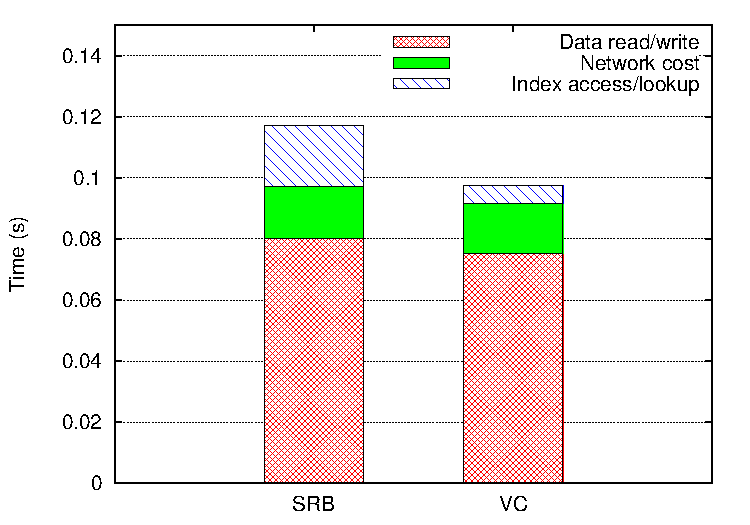
\epsfig{file=figures/srb_vs_vc, width=3in}
%   \caption{Time to backup a dirty VM segment under SRB and VC}
%   \label{fig:srb_vs_vc}
% \end{figure}


% \begin{figure}
%     \centering
%     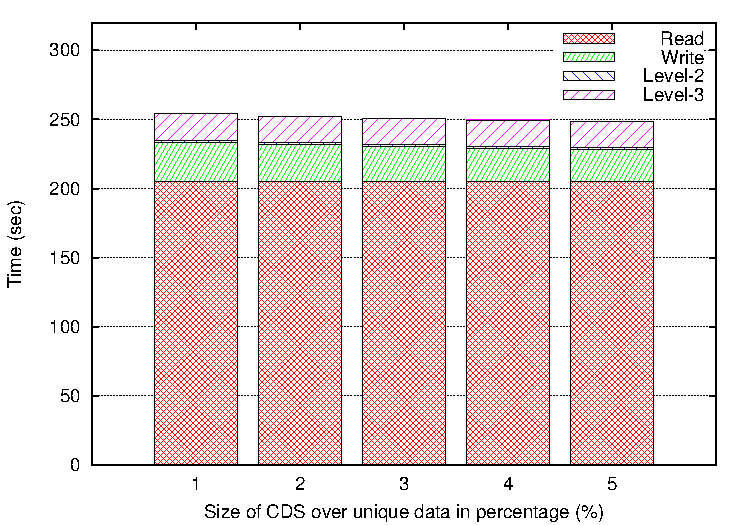
\includegraphics[width=3in]{figures/single_backup_time}
%     \caption{Average time to backup a VM in VC with varying PDS sizes}
%     \label{fig:single_vm_backup}
% \end{figure}


% \begin{table*}[t]
%     \centering
%     \begin{tabular}{c|ccc|ccc}
%     Num. of concurrent      & \multicolumn{3}{c|}{Throughput without}    & \multicolumn{3}{c}{Throughput with} \\
%     backup tasks            & \multicolumn{3}{c|}{I/O throttling (MB/s)} & \multicolumn{3}{c}{I/O throttling (MB/s)} \\ \cline{2-7}
%     per node                & Raw                                        & Snapshot Store & QFS  & Raw                                    & Snapshot Store & QFS  \\ \hline
%     1                       & 1369.6                                     & 148.0          & 18.0 & 171.3                                  & 18.5           & 2.26 \\
%     2                       & 2408.5                                     & 260.2          & 31.7 & 201.3                                  & 21.8           & 2.66 \\
%     4                       & 4101.8                                     & 443.3          & 54.1 & 217.8                                  & 23.5           & 2.87 \\
%     6                       & 5456.5                                     & 589.7          & 72.0 & 224.1                                  & 24.2           & 2.96 \\
%     \end{tabular}
% \caption{Throughput of software layers under different concurrency}
% \label{tab:throughput}
% \end{table*}
%\begin{table}[htbp]
\begin{table}[t]
  \centering
    \begin{tabular}{|c|ccc|}
\hline
    Concurrent      & \multicolumn{3}{c|}{Throughput without}    \\
    backup tasks            & \multicolumn{3}{c|}{I/O throttling (MB/s)} \\ \cline{2-4}
    per machine                & Backup                                     & Snapshot Store & QFS  \\ 
    		&                                      & (write) & (write)  \\ \hline
    1                       & 1369.6                                     & 148.0          & 35.3 \\
    2                       & 2408.5                                     & 260.2          & 61.7 \\
    4                       & 4101.8                                     & 443.3          & 103.1 \\
    6                       & 5456.5                                     & 589.7          & 143.8 \\ \hline
    \end{tabular}
\caption{Throughput of software layers per machine under different concurrency and without I/O throttling.}
\label{tab:throughput}
\end{table}

{\bf Throughput of software layers without I/O throttling.}
Table~\ref{tab:throughput} shows the  average throughput of software layers
when I/O throttling is not applied to control usage. The
%machine when all machine nodes execute one or multiple MV backup tasks.
``Backup'' column is the throughput  of the backup service  per machine.
``Snapshot store" is the  write throughput of the snapshot store layer and the significant reduction from this
column to  ``Backup" column is caused by deduplication.
Only non-duplicate chunks trigger a snapshot store write.
Column ``QFS'' is the write request traffic to the underlying file system after compression.
For example, with 148 MB/s write traffic to the snapshot store, QFS write traffic is about 35.3 MB/s
after compression.  However, the underlying disk storage traffic will be three times greater with replication.
The result shows that the backup service can deliver up to 5.46 GB/s 
per machine without I/O restriction
under 6 concurrent backup tasks. 
For our dataset, each version of total snapshots has abut 1TB per machine for 25 VMs and  thus  each machine
would complete the backup in about 3.05 minutes.
With a higher disk storage bandwidth available, the above backup
throughput would be higher. 
In comparison, the sampled index method in~\cite{Guo2011} achieves about 5.5GB per second
with 16 concurrent backup tasks and 6GB per second with
more tasks.  Thus the per-machine throughput of our scheme is reasonable.
%With 50MB/second controlled I/O bandwidth, each machine can deliver 171MB/second with 1 backup task and can complete the backup of 25 VMs per machine in less than 1.31 hours.
 
%To begin, on each node we write snapshots for 4 VMs concurrently, and gradually 
%increase number of VMs to 12 to saturate our system capability. 
%We observed 
%the per-node throughput peaked at 2700 MB/s when writing 10 VM snapshots in parallel, 
%which is far beyond our QFS file system capability. The reason behind it is our efficient
%deduplication architecture and compression which greatly reduce the amount of data that needs to be written to
%the file system. The main bottleneck here is that our QFS installation only
%manages one disk per node, which prevents it from fully utilizing the
%benefits of parallel disk access. We expect our architecture can
%perform even better in production clusters, which often have ten or more disks on each node.


% \begin{figure}
%     \centering
%     \subfigure[Backup throughput per node under controlled I/O bandwidth usage]
%     {
%         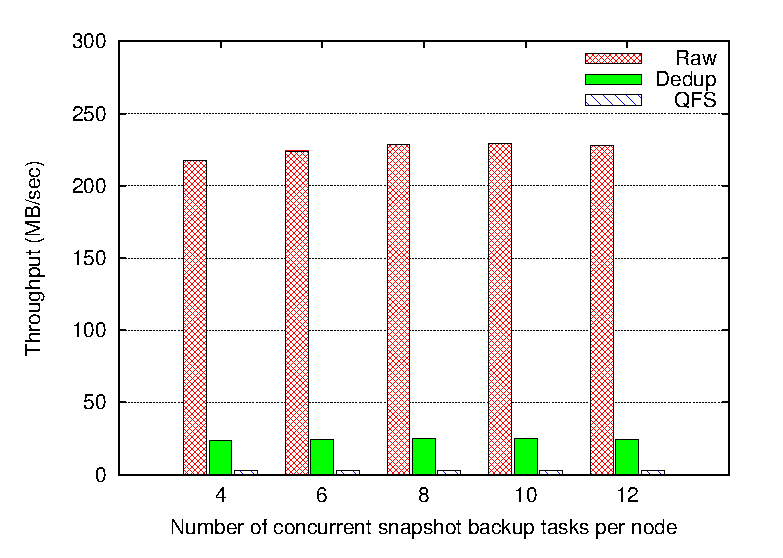
\includegraphics[width=3in]{figures/parallel_backup_with_read}
%         \label{fig:withread}
%     }
%     \\
%     \subfigure[Deduplication and storage system performance]
%     {
%         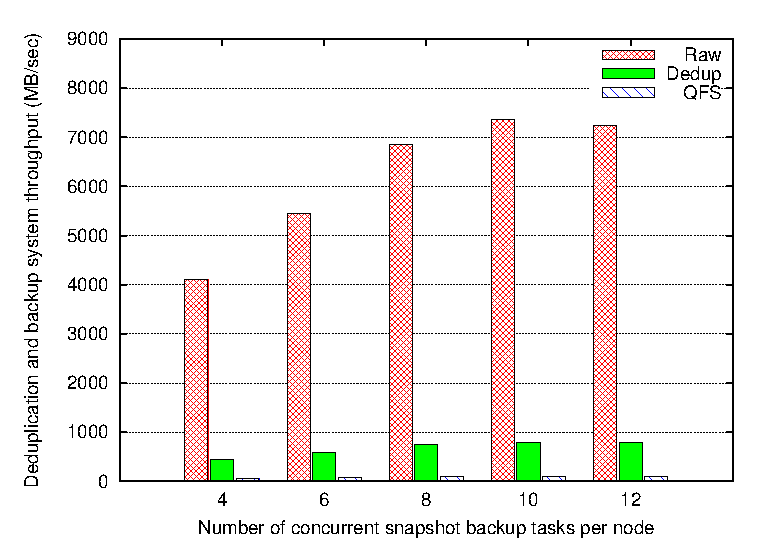
\includegraphics[width=3in]{figures/parallel_backup_no_read}
%         \label{fig:noread}
%     }
%     \caption{Throughput per-node with concurrent snapshot backup tasks}
%     \label{fig:parallel_backup}
% \end{figure}

 \subsection{Effectiveness of Approximate Deletion}



\begin{table}[htb]
\centering
\begin{tabular}{|c|c|c|c|}
    \hline 
%& \multicolumn{4}{|c|}{VC}  & VO \\ \hline
	    &Time p=50 & Time p=100 & Memory \\
	    &(hours)  & (hours) & (GB) \\
\hline
Mark-sweep  & 35.9  &  84.3  & 1.2--3 \\
\hline
Grouped &     18.6    & 43.6   & 1.2--3 \\
mark-sweep &        &    &  \\
\hline
VC w/o sum &  0.7     & 0.82   & 0.05 -- 1.96 \\
\hline
VC  &  0.012      & 0.014   & 0.015  \\
\hline
\hline
VC Repair  &  0.7      & 0.82   & 0.05 -- 1.96 \\
\hline
    \end{tabular}
    \caption{ Processing time and per-machine memory usage  for
deletion}  
    \label{tab:deletion-cmp}
\end{table}

Table~\ref{tab:deletion-cmp}   lists a comparison of processing time and memory usage
using the four deletion approaches when $p=100$ and $p=50$. These four 
methods are 1) the standard mark-sweep method. 2) Grouped mark-sweep~\cite{Guo2011}. 
3)   VC summary vectors. 4) VC with summary vectors.
The I/O speed for the backend distributed file system is about 50MB/second
and the speed drops to about 25MB/second when
when 100 machines read the backend file system concurrently due to the network
contention. We explain the results for $p=100$ below and notice each physical machine hosts 25VMs on average. The explanation for $p=50$ is similar.

For the mark-sweep approach on $p=100$, a physical machine is responsible for
reading the metadata of non-deduplicated chunks used in the hosted 
virtual machines and keeping the usage index table in the memory.
Then all machines read the meta data 
of snapshots in parallel and mark the usage of referenced chunks
in the usage table.
This process is repeated 100 times (once for for each physical machine).
The memory allocated at each physical machine is for the 
chunk usage table of 25 VMs. The average size is 1.2GB and the maximum is
3GB in our dataset. If we reduce the size of  the usage table at each machine, 
then there are more iterations to mark all data and it 
will take more time.    
For the grouped mark-sweep, about 50\% of snapshot metadata reading can be 
avoided in assessing the reference usage of non-duplicate chunks. 
Thus it takes 50\% less time, which is about 43 hours, but the 
memory requirement does not decrease.

For VC without summary vectors, all physical machines conduct the mark-sweep process in parallel, 
but each machine only handles one VM at time and 
the scope of meta data comparison is controlled within the single VM.
Popular chunks are excluded. The average memory usage is the index size of 
non-deduplicated VM chunks, which is about 50MB on average and the largest
size is 1.96GB. 
For VC with summary vectors, each physical machine loads
the VM snapshots and only needs to compare with the summary vectors.
The memory usage is controlled within 15MB for hosting the summary vectors
and small buffers. The deletion time is reduced to less than 1 minute.
The periodic leakage repair still takes about 0.83 hours while using
an average of 50MB memory. For  few big VMs in a skewed data distribution,
the repair uses upto 1.9GB memory.
Such a repair does not occur often (e.g. occurs every 19.6 days as discussed in Section~\ref{sect:delete}). 



\comments{
 \begin{figure}
\vspace{-0.1in}
     \centering
     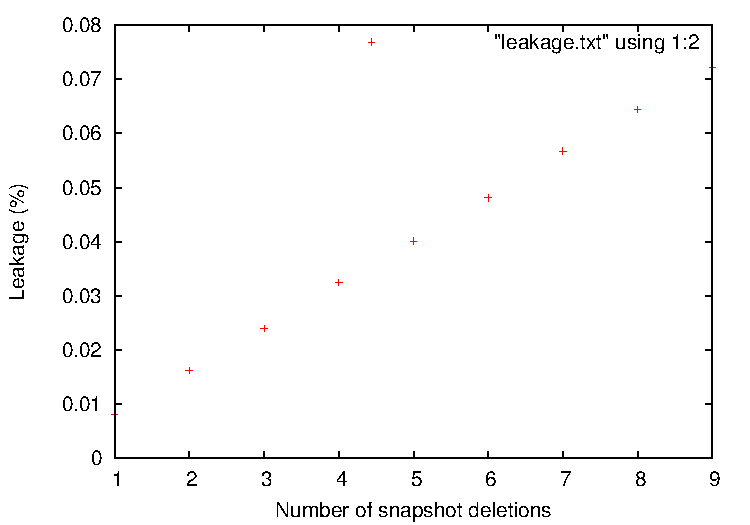
\includegraphics[width=3in]{figures/leakage}
     \caption{Accumulated storage leakage by approximate snapshot deletions ($\Delta u/u=0.025$)}
     \label{fig:leakage}
 \end{figure}
}
\begin{table}
\centering
    \begin{tabular}{|c|c|c|c|c|c|}
    \hline
Del. step   &     1 &  3  & 5 & 7  & 9 \\ 
\hline   
     Estimated& .02\% & .06\% & .10\%& .14\% & .18\%\\ 
\hline   
     Measured & .01\% & .055\% & .09\% & .12\% & .15\% \\
\hline   
    \end{tabular}
     \caption{Accumulated storage leakage by approximate snapshot deletions ($\Delta u/u=0.025$)}
     \label{tab:leakage}
\end{table}

Table~\ref{tab:leakage} shows the average accumulated storage leakage in terms of percentage of
storage space per VM caused  by approximate deletions.
In this experiment, we select 105 VMs and let all the VMs accumulate 10 snapshots, 
then start to delete those snapshots one by one in reverse order.
As we know the actual storage needs after each snapshot creation,
the storage leakage can be detected by
comparing the size of remaining data in use after deletion to the correct number.
Row 1 in  Table~\ref{tab:leakage} 
is the deletion step. Entry value 3 in this row   means that Version 3 is deleted. 
Row  2 is the predicted leakage using Formula~\ref{eq:leakrepair} from Section~\ref{sect:delete}
given $\Delta u/u=0.025$,
while Row 3 lists the actual average leakage measured during the experiment for all the VMs. 
The Bloom filter setting is based on $\Delta u/u=0.025$.
After 9 snapshot deletions, the actual leakage ratio reaches 0.0015 and this means that
there is only 1.5MB space leaked for every 1GB of stored data.
The actual leakage can reach  4.1\% after  245 deletions.
% and such a repair is needed every 12 days to the  leakage under 5\%. 
This experiment shows that the leakage of our approximate snapshot deletion is very small, 
below the estimated number.

\comments{
The space cost for each snapshot deletion is insignificant.
Leakage repair for each VM needs less than 85MB of memory
considering each reference consumes 8 bytes plus  1 mark bit and  
each VM snapshot has 40GB backup data with about 10 million chunks. 
This VM-specific leakage  repair takes  less than half an hour for each VM. 
}
%when disk bandwidth is controlled to 50MB/s. 
%When using the traditional mark-and-sweep~\cite{Guo2011,Fabiano2013} in VO for 2500 VMs, 
%a total of 212GB memory
%space on 100 node is accessed for processing each VM and each machine requires 2.12GB.
%To control the garbage growth, such a process needs to be conducted much more frequently than our
%VM-centric leakage repair. 

%Assuming snapshot deletion happens daily,
%such a  mark-and-sweep deletion needs to be conducted every two days to control garbage space under 5\%
%since there is 2.5\% data change for each snapshot.


% We also measure the storage leakage under $\Delta u/u=0.05$ and $0.10$ settings for summary vectors.
% As this value increases, larger summary vectors are generated thus results in a decrease on the
% false-positive ratio, therefore less amount of unused chunks are misjudged. 

%\subsection{Fault Isolation and Snapshot Availability}
\subsection{Snapshot Availability}

We demonstrate  
%the impact of adding extra replication for PDS in VC
%and compare 
the snapshot availability of VC and SRB-based VO  when there are failed machines. 
Appendix~\ref{sect:fault} provides a detailed analysis of 
snapshot availability and the estimated result depends on how frequent a duplicate chunk
is shared among snapshots of VMs.
The trace driven execution allows us to estimate the number of file blocks shared by each VM in the VO 
and VC approaches
and then calculate the average availability of VM snapshots.

Table~\ref{tab:vm-availability} shows the estimated availability of VM snapshots when 
there are up to 20 machines failed in a cluster. 
The case for  a 1000-node cluster is also listed, assuming file block sharing patterns among VMs remain
the same from $p=100$ setting to $p=1000$. Each machine hosts about 25 VMs in both cases
and with different $p$ values, the availability varies when the number of failures in the cluster changes.

%Two VC curves use $V_c=1250$ and $V_c=2500$ representing the average number of VMs that share a PDS file system block. 
%We have assumed a worst-case scenario that  a PDS block is shared by every VM. 
%($V_c=p*V$), which is to be expected when PDS
%blocks are sorted by hash, as their order is randomized.
%$V_c=2500$ represents  the absolute worst case for 2500 VMs. 
%The VO curve has  $V_o=6.3$ which is the average number of VMs that share a file system block in our smaller dataset.
%To get this number, we perform perfect deduplication over 105 VMs, append unique chunks to a DFS file and
%count the number of dependencies from a file system block to VM.
%In the scenario of having 2500 VMs, this number can only increase, thus this number represents the best
%case for VO approach. 
%Our results show that the VC approach even with $V_c=2500$ has a higher availability than VO.
%For example, with 10 machines failed, VO with 98.5\% availability would lose snapshots of 37 VMs 
%while VC with 99.9\% loses snapshots of 2.5 VMs.
%The key reason is that  $N_1 +N_2 < N_o$, caused by the fact that the VM-centric approach localizes deduplication
%and packs  data blocks for one VM as much as possible.  The extra replication
%for PDS blocks also significantly increases the snapshot availability even when
%a PDS file block is shared by every VM.
%=======
%Figure~\ref{tab:vm-availability} shows the availability of VM snapshots
%as storage nodes fail. 
%We assume a random distirbution of 64MB file system
%blocks (FSBs). where FSBs are not randomly distributed availability might
%be improved by limiting the number of storage nodes a particualr VM depends
%on but we take the conservative approach. We compare VO, the expected case for
%VC ($V_c=p*V/2$), and the worst case for VC ($V_c=p*V/2$). We set $V_o=6.3$
%based on measured values in our dataset.
%To obtain VO sharing of file blocks, we perform perfect deduplication over 105 VMs, 
%append unique chunks to a DFS file and
%count the number of dependencies from a file system block to VM.
%In the case of having 2500 or even 25000 VMs, this number can only increase, thus this number represents the best
%case for VO approach. 


 Table~\ref{tab:vm-availability} shows 
that VC has a significantly  higher availability than VO.
% as the number of failed machines increases from 3 to 20.
%Our VM-centric approach shows significant improvements
%in VM availability.
With $p=100$ and 3 failures,
VO with 69.5\% availability could lose data in 763 VMs 
while VC with 99.7\% only loses data for 8 VMs out of 2500 VMs.
The key reason is that for most data in VC, only a single VM can be affected by
the loss of a single file block
%Since most blocks contain chunks for a single
%VM, VMs can depend on a smaller number of blocks, 
while in VO, the loss of a
single block tends to affect many VMs.
When the number of physical machines failed reaches 20, the availability of VO reaches 0\%
and VC also drops to 1.13\%. This is because even there is a good availability for PDS data, VC still
loses most of non-PDS blocks given the replication degree for non PDS is 3.
When $p=1000$, the percentage of failures is then 2\% and VC delivers a meaningful availability 
with 99.62\%, outperforming VO significantly. 

% because our VM-centric approach
%localizes deduplication.  

%Although the loss of a PDS block affects many VMs,
%by increasing replication for those blocks we minimize the effect on VM
%snapshot availability, and this is one of the key contributions of our
%approach, the clear separation of highly popular data from less popular data.

%By having extra replicas for the PDS data, we reduce the failure rate of PDS
%FSBs enough that the failure rate for the VM approaches the failure rate of the
%Non-PDS blocks. This minimizes the drop in availability between the expected
%and worst case for VC.
%
%One of the advantages of VC is that there is a division between
%popular and non-popular data to facilitate improved reliability. 
Figure~\ref{fig:pds-replication} shows
the impact of increasing PDS data replication degree. 
While the impact on storage cost is small (because we have separated out only
the most popular blocks),
a replication degree of 6  has a significant improvement over 4. The
availability does not increase much  when increasing
$r_c$ from 6 to 9 and the benefit is not so visible after $r_c>9$. 
That is because when the number of failed machines increases beyond 6, 
the non-PDS data availability starts to deteriorate significantly given its replication degree
$r$ is set to 3. Thus when $r=3$, the reasonable choice for $r_c$ would be a number between 6 and 9.
 
%This is because, as described before, the availability of the VM approaches the
%availiability of the Non-PDS data as the failure rate of PDS data gets very small.


\begin{table}[htbp]
  \centering
    \footnotesize
    \tabcolsep=0.11cm
    \pgfplotstabletypeset[
        comment chars=!,%use ! before a row in the data table to exclude it
        columns={NodesFailed,VO100,VC100,VO1000,VC1000},
        columns/NodesFailed/.style={
            column name={\multirow{3}{*}{Failures ($d$)}}
        },
        columns/VO100/.style={
            column name={
                \multicolumn{4}{c|}{VM Snapshot Availability(\%)}\\&
                \multicolumn{2}{c|}{$p=100$}&\multicolumn{2}{c|}{$p=1000$}\\&
            VO},
            fixed, precision=6
        },
        columns/VC100/.style={
            column name={VC},
            fixed, precision=6},
        columns/VO1000/.style={
            column name={VO},
            fixed, precision=6},
        columns/VC1000/.style={
            column name={VC},
            fixed, precision=6},
        every head row/.style={
            before row={\hline},
            after row={\hline},
        },
        every last row/.style={after row=\hline},
        column type/.add={}{|},
        every first column/.style={column type/.add={|}{}},
        %the below rows can be used to extract rows 3,5,10,20 from rows 0-40
        %skip rows between index={0}{3},
        %skip rows between index={4}{5},
        %skip rows between index={6}{10},
        %skip rows between index={11}{20},
        %skip rows between index={21}{41}
    ]{figures/availability_table.txt}
    \caption{Availability of VM snapshots for VO ($r=3$) and VC ($r_c=6$, $r=3$).}
    \label{tab:vm-availability}
\end{table}

\begin{figure}[htbp]
  \centering
	\begin{tikzpicture}
		\begin{axis}[
                        width=\linewidth,
                        height=0.6\linewidth,
		%title={PDS Replication affect on availability},
		xlabel={Failed storage nodes},
		ylabel={Availability (\%)},
                xmin=0,
                xmax=10,
		%extra y ticks={99.9}, %if important numbers are missing
                mark options=solid,
                legend style={
                    cells={anchor=west}, %legend entry alignment
                    legend pos=south west %legend position
                },
                reverse legend,
		]
                \addplot+[dashed] table[x=NodesFailed,y=VO]{figures/node_failures_100.txt};
                \addplot table[x=NodesFailed,y=VC1]{figures/node_failures_100.txt};
                \addplot table[x=NodesFailed,y=VC2]{figures/node_failures_100.txt};
                \addplot table[x=NodesFailed,y=VC3]{figures/node_failures_100.txt};
                \addplot table[x=NodesFailed,y=VC4]{figures/node_failures_100.txt};
                \legend{
                    VO,
                    $r_c=4$,
                    $r_c=5$,
                    $r_c=6$,
                    $r_c=9$
                }
		\end{axis}
	\end{tikzpicture}
  \caption{Availability of VM snapshots in VC with different PDS replication degrees on a $p=100$-node cluster.}
  \label{fig:pds-replication}
\end{figure}



